\documentclass[reading]{hitrep}

\usepackage{tabularx}
\newcolumntype{C}{>{\centering\arraybackslash}X}

\subject{人工智能原理及应用}
\department{计算学部}
\major{计算机技术}
\author{胡冠宇}
\studentid{24S103184}
\studenttype{硕士研究生}

\newcounter{csubsection}
\NewDocumentCommand\optmodule{sO{}mmm}{%
    \IfBooleanTF{#1}{%
        \begin{equation*}
            \ifthenelse{\equal{#2}{}}{}{(#2)\quad}
            \begin{aligned}
                \begin{cases}
                    #3 \quad & #4 \\
                    \mathrm{s.t.} \quad #5
                \end{cases}
            \end{aligned}
        \end{equation*}
    }{%
        \begin{equation}
            \ifthenelse{\equal{#2}{}}{}{(#2)\quad}
            \begin{aligned}
                \begin{cases}
                    #3 \quad & #4 \\
                    \mathrm{s.t.} \quad #5
                \end{cases}
            \end{aligned}
        \end{equation}
    }%
}

\begin{document}
    % \nocite{*}

    \maketitle

    \section{问题介绍}

\subsection{基于跨域表示学习的工业控制系统异常检测}

工业控制系统广泛应用于电力、制造、水利等关键基础设施,其安全性和稳定性至关重要。
一旦ICS受到攻击,可能会造成严重的损坏。
因此,针对ICS异常检测是十分重要的。
传统异常检测方法主要关注单一域中的指标,如网络域中的网络流量或物理域中的传感器数据,但ICS中不同域(如传感器的物理状态、网络通信流量等)的行为存在强相关性,仅分析单一域难以全面识别异常。
例如,网络攻击可能导致传感器数据异常,但某些攻击仅影响物理设备而不改变网络流量。
现有的方法如基于RNN\cite{mandic2001recurrent}、GAN\cite{creswell2018generative}或基于单域图的神经网络模型无法有效建模跨域关联,导致检测精度不足和误报率高。
文章\cite{zhan2024anomaly}在GDN\cite{deng2021graph}的基础上提出了一种基于跨域表示学习的ICS异常检测方法(MGDN),该方法能够学习多域行为的联合特征,并在不同的域内进行异常检测。
在构建跨域图来表示ICS中多个领域的行为之后,该方法可以利用图神经网络学习它们的联合特征。
由于异常在不同领域表现不同,利用多任务学习方法分别识别不同领域的异常并进行联合训练。

\subsection{基于异构图的大规模微服务系统性能问题诊断}

大规模微服务系统在运行过程中通常会产生大量的服务调用,尤其是在短时间内。
这意味着当检测到性能问题时,系统周围可能会有大量的调用记录。
这种海量的数据使得分析所有调用记录变得既低效又困难,而且根因定位的精度也会受到影响。
主要原因在于,其中许多服务调用与性能问题并无直接关系。
因此需要识别与性能问题有关的微服务调用。

大多数传统的方法识别异常的调用端口(即端口级),文章\cite{tao2024diagnosing}提出了一种基于服务级的异常检测方法(MicorDig)。
为了更准确地定位异常微服务,文章首先选择构建端口级调用图,然后,通过在图上执行广度优先搜索(Breadth-First Search,BFS)和异常检测来保留相关调用和相应的微服务。
如\cref{img:Port-level call graph}所示,圆圈表示端口级节点,同一个虚线椭圆内的端口属于同一个微服务,橙色的端口级节点为问题无关节点,虚线表示的调用为非异常调用。
最后,如\cref{img:Service-level call graph}所示,将图中的端口级节点聚合到服务级。

\begin{figure}[ht]
    \centering
    \begin{subfigure}{0.32\linewidth}
        \centering
        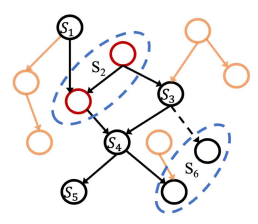
\includegraphics[scale = 0.6]{img/port-level call graph.png}
        \caption{端口级调用图}
        \label{img:Port-level call graph}
    \end{subfigure}
    \begin{subfigure}{0.32\linewidth}
        \centering
        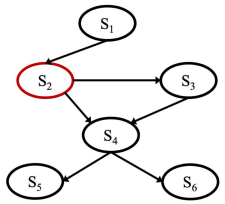
\includegraphics[scale = 0.6]{img/Service-level call graph.png}
        \caption{服务级调用图}
        \label{img:Service-level call graph}
    \end{subfigure}
    \begin{subfigure}{0.32\linewidth}
        \centering
        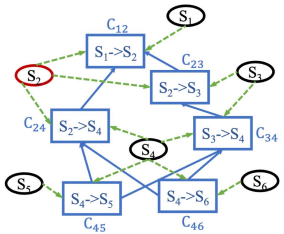
\includegraphics[scale = 0.55]{img/Service-level Heterogeneous Propagation Graph.png}
        \caption{服务级异构传播图}
        \label{img:Service-level Heterogeneous Propagation Graph}
    \end{subfigure}
    \caption{异构传播图的构造过程}
\end{figure}

    \section{相关求解算法简介及其实现}

\subsection{MGDN}

文章提出一种跨域图表示学习方法。
核心思想是通过构建多域图结构,将不同域的行为特征统一编码。
该方法结合不同域的数据,利用注意力机制图卷积网络(Graph Convolutional Networks,GCN)\cite{kipf2017semi}学习共享与域特定特征。
模型框架如\cref{figure:跨域表示学习的总体框架}所示。

\begin{figure}[ht]
    \centering
    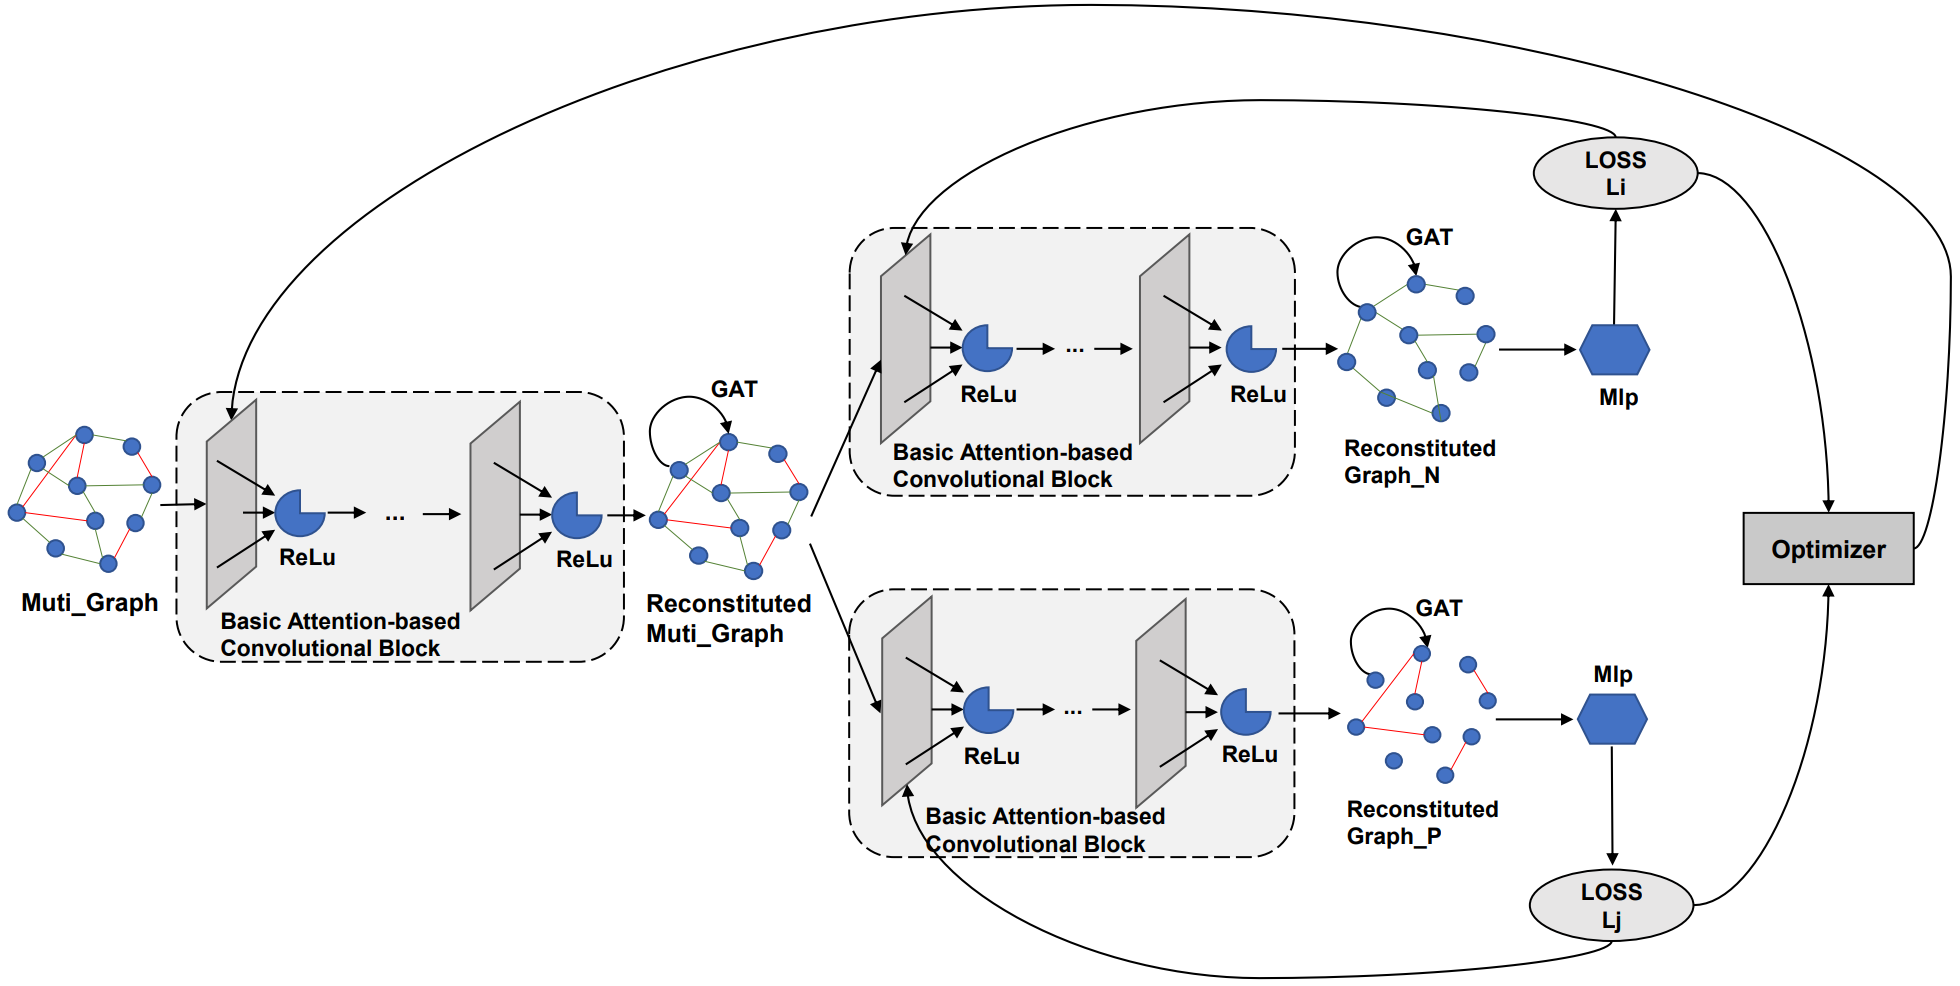
\includegraphics[width=1\textwidth]{img/跨域表示学习的总体框架.png}
    \caption{跨域表示学习的总体框架}
    \label{figure:跨域表示学习的总体框架}
\end{figure}

\subsubsection{多图构建}

在该方法中,目标是从ICS的多个域(如物理域、网络域等)中提取节点特征,并构建统一的多图结构用于跨域建模。
多图表示结构的构构建过程如\cref{figure:多图表示结构的构建过程}所示。

\begin{figure}[ht]
    \centering
    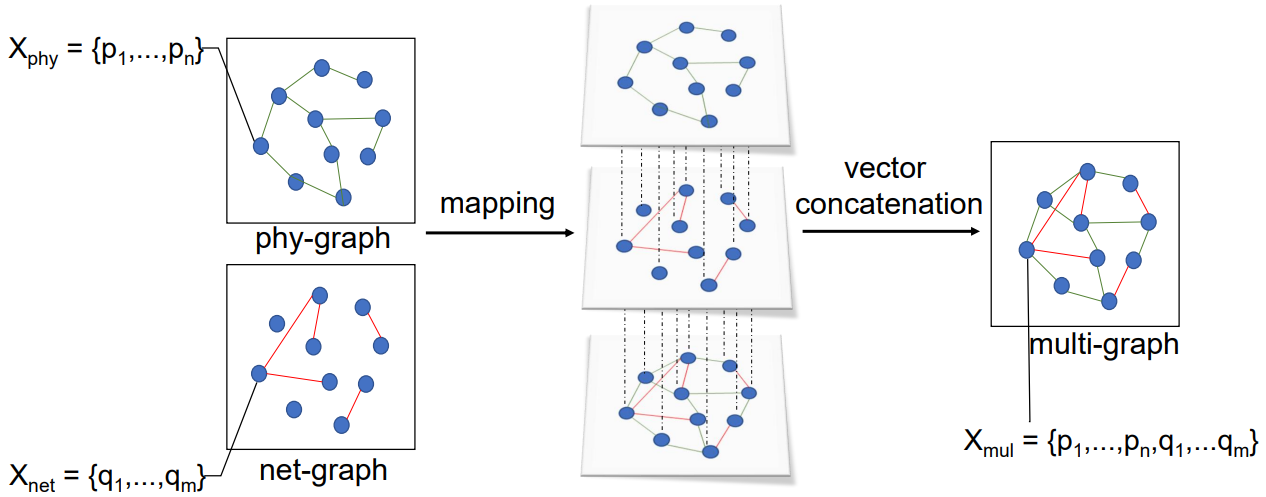
\includegraphics[width=1\textwidth]{img/多图表示结构的构建过程.png}
    \caption{多图表示结构的构建过程}
    \label{figure:多图表示结构的构建过程}
\end{figure}

假设有$n$个节点(传感器和执行器),来自不同域的数据被统一为相同的时间粒度(如秒级粒度),每个节点在第$d$个域上的特征矩阵为
\begin{equation*}
    \bm{x}^{(d)}\in\mathbb{R}^{n\times t} \text{,}
\end{equation*}
其中$t$为时间步长。

对每个域$d\in\{1,2,\cdots,D\}$, 构建一个无向加权图
\begin{equation*}
    \mathcal{G}_d=\left<\mathcal{V},\mathcal{E}_d\right> \text{,}
\end{equation*}
其中$\mathcal{V}$表示所有节点的集合,且$|\mathcal{V}|=n$,$\mathcal{E}_d$为第$d$个域中的边集合。

节点之间的边权通过余弦相似度计算其嵌入向量之间的相似性。
对于任意两个节点$i$和节点$j$,在第$d$域的嵌入向量为$\bm{v}_i^{(d)}$和$\bm{v}_j^{(d)}$,则计算节点$i$到节点$j$的边权
\begin{equation*}
    e_{ij}^{(d)}=\frac{\left(\bm{v}_i^{(d)}\right)^\mathrm{T}\bm{v}_j^{(d)}}{\left\|\bm{v}_i^{(d)}\right\|\left\|\bm{v}_j^{(d)}\right\|} \text{,}
\end{equation*}
之后使用Top-k策略筛选每个节点最相关的$k$个邻居构建图$\mathcal{G}_d$,进一步融合成多图结构
\begin{equation*}
    \mathcal{G}=\left<\mathcal{V}, \textstyle\bigcup_{i=1}^d\mathcal{E}_i\right> \text{,}
\end{equation*}
节点$i$的跨域特征向量表示为
\begin{equation*}
    \bm{v}_i=\bm{v}_i^{(1)}\oplus\bm{v}_i^{(2)}\oplus\cdots\oplus\bm{v}_i^{(D)} \text{。}
\end{equation*}

\subsubsection{基于注意力的图卷积建模}

该部分通过引入图注意力机制(Graph Attention Network, GAT)\cite{deng2021graph}对节点信息进行聚合,捕捉局部邻居中的非均匀关系。

首先,定义节点$j$对节点$i$的注意力权重
\begin{equation*}
    \alpha_{ij}=\mathrm{Softmax}\left(\mathrm{LeakeyReLU}\left(\bm{a}^\mathrm{T}(\bm{v}_i\oplus\bm{v}_j)\right)\right) \text{,}
\end{equation*}
其中$\bm{a}$为可学习的向量。则节点$i$的表示更新为
\begin{equation*}
    \bm{z}_i=\mathrm{ReLU}\left(\alpha_{ii}\bm{W}\bm{v}_i+\bm{W}\sum_{j\in\mathcal{N}_i}\alpha_{ij}\bm{v}_j\right) \text{,}
\end{equation*}
其中$\bm{W}$为可学习的矩阵。

使用节点的聚合表示和特征向量进行输出,即
\begin{equation*}
    \hat{\bm{y}}=f_\theta([\bm{z}_1\circ\bm{v}_1, \bm{z}_2\circ\bm{v}_2, \cdots, \bm{z}_n\circ\bm{v}_n]) \text{,}
\end{equation*}
其中$\circ$为逐元素乘法,$f_\theta$为多层感知机。


\subsubsection{多目标优化}

为了在多个域(如物理域、网络域等)上同时优化预测性能,文章使用了多任务学习(Multi-Task Learning, MTL)方法,其目标是联合优化每个任务的损失
\begin{equation*}
    \min_{\bm{W}_s,\bm{W}_1,\bm{W}_2,\cdots,\bm{W}_D}\sum_{d=1}^D\gamma_d\mathcal{L}_d(\bm{W}_s,\bm{W}_d) \text{,}
\end{equation*}
其中$\bm{W}_s$为共享层参数,$\bm{W}_d$、$\mathcal{L}_d$和$\gamma_d$分别为第$d$域的专属参数、损失函数及任务权重。

为了解决梯度冲突问题,引入了多梯度下降算法(Multiple Gradient Descent Algorithm,MGDA)\cite{desideri2012multiple},其基本思想是寻找一组权重$\{\gamma_d\}$,使得多个损失函数在共享参数$\bm{W}_s$上的梯度方向可以共同优化,即
\optmodule{\min_{\gamma_1,\gamma_2,\cdots,\gamma_D}}{\left\|\sum_{d=1}^D\gamma_d\nabla_{\bm{W}_s}\mathcal{L}_d(\bm{W}_s,\bm{W}_d)\right\|^2}{
    &\sum_{d=1}^D\gamma_d=1\text{,} \\
    &\gamma_1,\gamma_2,\cdots,\gamma_D\geq0\text{,}
    \label{equation:MGDA}
}
该优化问题保证在共享参数更新中不会偏向某一特定任务。

文章中的$D=2$,因此\cref{equation:MGDA}可简化为
\optmodule*{\min_{\gamma}}{\left\|\gamma\nabla_{\bm{W}_s}\mathcal{L}_1(\bm{W}_s,\bm{W}_1)+(1-\gamma)\nabla_{\bm{W}_s}\mathcal{L}_2(\bm{W}_s,\bm{W}_2)\right\|^2}{
    &\gamma\geq0\text{。}
}

\subsection{MicroDig}

为了捕捉性能问题的传播模式并进一步缩小候选根本原因的范围,文章对关联图中的每一条边执行异常检测,使用一种高效且广泛使用的异常检测方法——$k$-$\sigma$方法。
该方法从历史数据中学习参数$\mu$和$\sigma$,并将超出$(\mu-k\sigma,\mu+k\sigma)$范围的值视为异常。

文章基于端口级数据进行异常检测,而不是基于服务级数据,因为端口级的异常可能意味着包含该端口的服务存在异常行为,如果基于从端口级数据汇总的服务级数据进行异常检测,可能会被这些异常淹没。
根据上述步骤,文章保留了关联图中存在异常的边。
由于通过上述步骤得到的图是端口级关联图,而文章的目标是定位异常服务,因此需要合并端口的调用数据,并构建服务级关联图。

令$p$为端口级关联图中的一个节点,用$P(S)$表示给定服务$S$的所有端口。
为了构建服务级图,需要将同一服务$S$的所有端口级节点合并为一个节点,记为$S = \{p\in P(S)\}$。在服务级图上,边$S\to^{call}S'$的异常率$R(S, S')$整合了每个相关端口级边$p\to^{call}p'$的异常调用数$F(p, p')$和总调用数$N(p, p')$,即对于时间节点$t$,有
\begin{equation*}
    R_t(S, S')=\frac{\displaystyle\sum_{p\in S,p'\in S'}F_t(p,p')}{\displaystyle\sum_{p\in S,p'\in S'}N_t(p,p')}
\end{equation*}

通过上述步骤,可以构建一个服务级关联图,其中的节点都与问题服务相关。
同时,可以获得边$S = \{p\in P(S)\}$的异常率时间序列:
\begin{equation*}
    R(S,S')=(R_{t-\varphi},R_{t-\varphi+1},\cdots,R_{t+\varphi})
\end{equation*}
该时间序列表示在时间区间$[t-\varphi,t+\varphi]$之间中边$S\to^{call}S'$的异常率变化。
MicroDig的总体框架如\cref{figure:MicroDig的总体框架}所示。

\begin{figure}[ht]
    \centering
    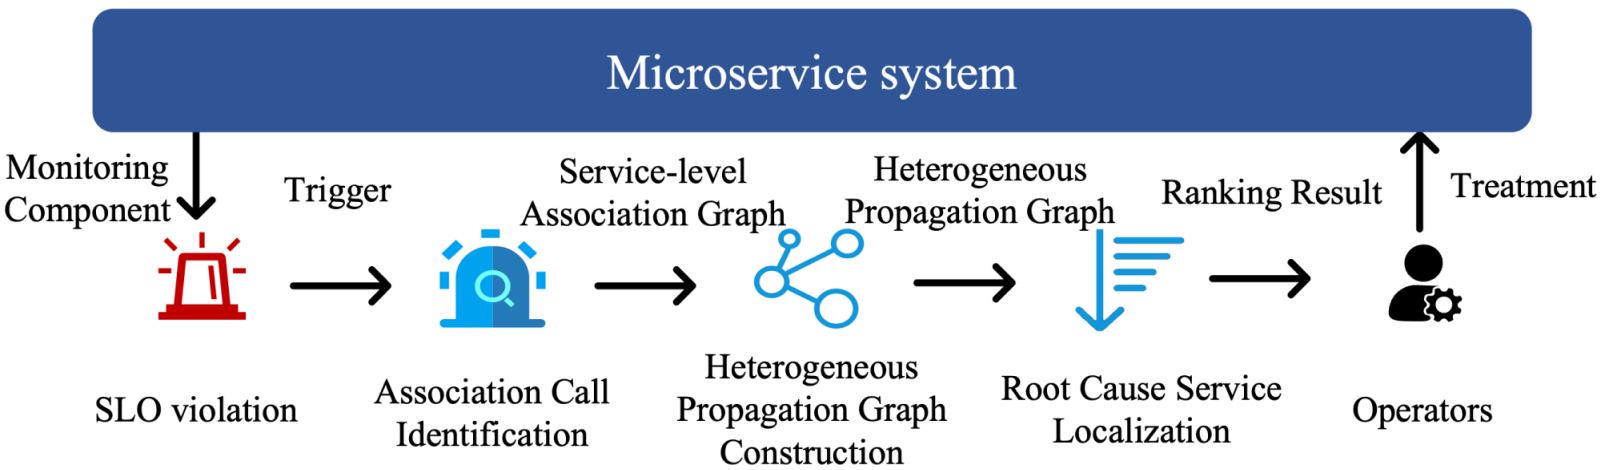
\includegraphics[width=\textwidth]{img/MicroDig框架.png}
    \caption{MicroDig的总体框架}
    \label{figure:MicroDig的总体框架}
\end{figure}

\subsubsection{异构传播图的构造}

构建的关联图是有向图,其边的方向表示服务之间的调用关系。
然而,调用关系并不等同于因果关系。
因此,关联图不能直接用作根本原因定位的因果图。
文章提出构建一个异构传播图,以反映调用和服务之间的因果关系,基于关联图进行构建。

\begin{algorithm}[!ht]
    \caption{异构传播图构造}
    \label{alg:Heterogeneous Propagation Graph Construction}
    \begin{algorithmic}[1]
        \State$G_h$\Get 初始化异构传播图
        \State$G_h$.addNodes($G$.edges())

        \ForAll{$S\in G$.nodes()}
            \ForAll{$C_{out}\in G$.outEdges($S$)}
                \ForAll{$C_{in}\in G$.inEdges($S$)}
                    \State $G_h$.addEdge($C_{out}$, $C_{in}$)
                \EndFor
            \EndFor
        \EndFor

        \State $G_h$.addNodes($G$.nodes())
        \ForAll{$C\in G$.edges()}
            \State $caller$, $callee$\Get\Call{splitCall}{$C$}
            \State $G_h$.addEdge($caller$, $C$)
            \State $G_h$.addEdge($callee$, $C$)
        \EndFor
    \end{algorithmic}
\end{algorithm}

\subsubsection{根因定位}

为了在异构传播图中进行根因定位,文章提出了一种新颖的方法,称为异构导向随机游走(Heterogeneity-Oriented Random Walk, HORW)。
该方法充分考虑了异构性的特点,并在转移概率的计算上进行了创新。
HORW方法的核心思想是通过模拟在异构传播图中的随机游走过程来识别根本原因。
与传统的随机游走方法不同,HORW不仅考虑了图中的节点和边的结构信息,还结合了不同类型的节点(如服务节点、调用节点)和边(如服务间调用、调用节点之间的因果关系)的异构特性。
通过对每种类型的边和节点赋予不同的权重,HORW能够更加精确地捕捉性能问题的传播路径,从而准确定位到根本原因服务。
该方法的创新之处在于转移概率的计算,即根据图中节点的类型和关联的边的性质来调整转移概率,而不是简单地依赖于图的结构。
这使得HORW能够更有效地识别和定位性能问题的根源,尤其是在复杂和动态的微服务环境中。

    \section{最新发展、数据集与SOTA结果}

\subsection{MGDN}

文章使用SWaT(Secure Water Treatment)\cite{mathur2016swat}数据集进行实验。
该数据集由新加坡科技设计大学(Singapore University of Technology and Design,SUTD)网络安全研究中心的iTrust实验室发布,模拟了真实水处理系统的运行场景。
数据集包含51个物理传感器(如流量计、阀门状态)和16个网络特征(如数据包数量、协议类型),时间跨度为11天,前7天为正常操作,后4天注入41种攻击。
\cref{table:swat static info}总结了SWaT数据集在物理和网络领域的统计数据。

\begin{table}[ht]
    \centering
    \caption{SWaT数据集在不同域中的统计数据}
    \label{table:swat static info}
    \begin{tabular}{ccccc}
        \toprule
        \textbf{域} & \textbf{训练数据} & \textbf{训练数据条目} & \textbf{特征数} & \textbf{异常率} \\
        \midrule
        物理域 & 21,830 & 34,201 & 51 & 16.61\% \\
        网络域 & 21,830 & 34,201 & 3  & 16.61\% \\
        \bottomrule
    \end{tabular}
\end{table}

文章使用准确率(Precision)、召回率(Recall)、假阳性率(False Positive Rate,FPR)和F1分数评估模型性能,这些指标的计算公式如下:
\begin{align*}
    &\mathrm{Precision}=\frac{\mathrm{TP}}{\mathrm{TP}+\mathrm{FP}} \text{,} \\
    &\mathrm{Recall}=\frac{\mathrm{TP}}{\mathrm{TP}+\mathrm{FN}} \text{,} \\
    &\mathrm{FPR}=\frac{\mathrm{FP}}{\mathrm{FP}+\mathrm{TN}} \text{,} \\
    &\mathrm{F1}=\frac{2\times\mathrm{Precision}\times\mathrm{Recall}}{\mathrm{Precision}+\mathrm{Recall}} \text{。}
\end{align*}
实验结果如\cref{table:matrics of mgdn and the baseline methods}所示。

\begin{table}[ht]
    \centering
    \caption{MGDN与基线方法的准确性(在数据集SWaT下)}
    \label{table:matrics of mgdn and the baseline methods}
    \begin{tabular}{ccccc}
        \toprule
        \textbf{Method} & \textbf{FPR (\%)} & \textbf{Precision (\%)} & \textbf{Recall (\%)} & \textbf{F1 (\%)} \\
        \midrule
        DTAAD       & 13.33 & 59.88 & 99.99 & 74.90 \\
        GDN         & 10.70 & 64.91 & 99.45 & 78.55 \\
        LSTM-AD     & 13.33 & 59.88 & 99.99 & 74.90 \\
        MAD-GAN     & 13.57 & 59.45 & 99.99 & 74.57 \\
        MSCRED      & 13.33 & 59.89 & 99.99 & 74.91 \\
        MTAD-GAT    & 13.39 & 59.78 & 99.99 & 74.83 \\
        OmniAnomaly & 13.36 & 59.83 & 99.99 & 74.87 \\
        TranAD      & 13.35 & 59.85 & 99.99 & 74.88 \\
        USAD        & 13.26 & 60.02 & 99.99 & 75.01 \\
        \textbf{MGDN}   & \textbf{3.07} & \textbf{84.65} & \textbf{85.12} & \textbf{84.88} \\
        \bottomrule
    \end{tabular}
\end{table}

\subsection{MicroDig}

在评估MicroDig的性能时,文章构建了三个数据集,分别是来自腾讯的真实世界性能问题案例(数据集$\mathcal{A}$)、开源微服务系统Train-Ticket中的注入问题(数据集$\mathcal{B}$)\cite{zhou2018fault},以及中国建设银行电子商务系统的模拟问题(数据集$\mathcal{C}$)。这些数据集涵盖了不同规模和类型的微服务系统,为全面评估MicroDig提供了丰富的场景。实验旨在回答三个研究问题:MicroDig的诊断准确性(RQ1)、诊断效率(RQ2)以及核心组件对性能的贡献(RQ3)。

\begin{table}[ht]
    \centering
    \caption{MicroDig与基线方法的准确性(在数据集$\mathcal{A}$下)}
    \label{table:the accuracy of microdig and the baseline methods A}
    \begin{tabular}{cccccc}
        \toprule
        \textbf{Method} & \textbf{AC@1 (\%)} & \textbf{AC@2 (\%)} & \textbf{AC@3 (\%)} & \textbf{Avg@3 (\%)} & \textbf{MRR} \\
        \midrule
        ServiceRank         & 50.8 & 55.7 & 57.4 & 54.6 & 0.55 \\
        MonitorRank         & 49.2 & 61.9 & 71.4 & 60.8 & 0.62 \\
        TraceRCA            & 61.5 & 72.7 & 75.8 & 70.0 & 0.70 \\
        TraceRank           & 16.9 & 20.3 & 20.3 & 19.2 & 0.20 \\
        Microscope          & 50.8 & 70.4 & 75.4 & 65.5 & 0.64 \\
        MicroHECL           & 61.9 & 73.8 & 76.2 & 70.6 & 0.71 \\
        \textbf{MicroDig}   & \textbf{64.4} & \textbf{87.3} & \textbf{94.1} & \textbf{81.9} & \textbf{0.78} \\
        \bottomrule
    \end{tabular}
\end{table}

文章选用了Top-$k$准确率(AC@k)、平均Top-$k$准确率(Avg@k)和平均倒数排名(MRR)作为主要的性能评估指标。这些指标能够全面反映MicroDig在定位性能问题根源时的准确性和效率。为了进行公平比较,文章选择了六种具有代表性的基线方法,包括Microscope、ServiceRank、MicroHECL、MonitorRank、TraceRCA和TraceRank,这些方法在各自的领域都展现出了优越的性能。

实验结果表明,MicroDig在所有三个数据集上都显著优于基线方法。如\cref{table:the accuracy of microdig and the baseline methods A}所示,在腾讯的真实世界数据集上,MicroDig在AC@1、AC@2和AC@3上分别比其他方法高出4\%、18.3\%和23.5\%。此外,MicroDig的平均诊断时间最短,为24.72秒/案例,显示出良好的效率。消融实验进一步证实了异构传播图、超参数$\beta$和异常检测对MicroDig性能的显著贡献。
    \section{结论}

工业控制系统与微服务架构的异常检测与根因分析是保障现代工业与互联网应用稳定性的核心问题。
两篇论文通过跨领域图表示学习与潜在空间干预识别,为解决复杂系统中的多维度、异构性问题提供了创新方案。

文章\cite{zhan2024anomaly}提出了一种基于跨域表示学习的异常检测方法,该方法将多个域的ICS数据结合起来进行跨域学习和异常检测。
通过物理域与网络域数据的联合建模,克服了单领域分析的局限性。注意力机制与多任务优化的结合,使模型在保留领域特征的同时捕捉跨域关联。
文章在大规模的真实世界数据集上对模型进行了评估,实验结果表明文章的模型优于基准模型。
此外,文章的模型能够更好地平衡减少误报和提高异常检测精度之间的关系,提供了一个更实用和理想的ICS异常检测模型。

文章\cite{tao2024diagnosing}在微服务系统性能诊断领域做出了重要贡献。
它不仅提供了一种新的根因定位方法,还通过实际案例展示了该方法的有效性。
尽管存在一些局限性,但文章也已经详尽写出,这位未来的研究工作进行了初步的规划和奠定了基础。
MicroDig的出现,无疑为微服务系统的运维和性能优化提供了新的工具和思路,对于提高系统的可靠性和用户体验具有重要意义。
此外,这项研究也为学术界和工业界提供了新的研究方向,特别是在微服务架构日益普及的背景下,如何有效地诊断和解决性能问题,成为了一个亟待解决的挑战。
MicroDig的成功应用,为这一挑战提供了一个有力的解决方案,也为未来的研究和实践提供了宝贵的经验和启示。


    \stepcounter{section}
    \renewcommand{\refname}{\chinese{section}、参考文献}
    \bibliography{references}
\end{document}
 